discrepancies \documentclass[11pt, letterpaper]{article}
\usepackage[margin=1.25in,  marginparwidth=2.5cm, marginparsep=0.25cm]{geometry}

% \setlength{\textheight}{8.75in}
% \setlength{\oddsidemargin}{.125in}

% \setlength{\textwidth}{6.25in}
% \linespread{1.4}
\usepackage{graphicx}
\usepackage{chemmacros}
\usepackage{amsmath}
\usepackage{float}
\usepackage{gensymb}
\usepackage{multirow}
\usepackage{color}
\usepackage{wrapfig}
\usepackage{tabularx}
\usepackage{marginnote}
\bibliographystyle{unsrt}
\usepackage[font=small,labelfont=bf]{caption}
\author{N. Belliveau, G. Chure, J. Theriot, R. Phillips}

\begin{document}
\title{Supplemental Information: }
\maketitle

\section{Summary of Proteome Datasets.}

Here we briefly summarize the datasets that were considered for the work of the main
text. The goal of this section is to give an overview of each dataset
considered, including the main experimental details, and to provide a more
detailed look at how well each compares.

Table \ref{table:datasets} provides an overview of the proteomic datasets that
we found in the literature. These are predominately mass spectrometry-based,
with the exception of the work from Li {\it et al.} (2014) which used ribosomal
profiling, and the fluorescence-based counting done in Taniguchi {\it et al.}
(2010). The general strategy taken in these works is to quantify fractional
abundance of each protein and then to convert these to absolute abundance by
multiplying these fractions by the bulk measured total cellular protein
abundance. Note that the work of Peebo {\it et al.} (2014) did not perform any
measurement of cell count or volume, and thus were only able to report cellular
protein concentration.

Exceptions to this are found in Schmidt {\it et al.} and Taniguchi {\it et al.}.
A key distinction in the work of Schmidt {\it et al.} is that in addition to
determining relative abundance by mass spectrometry, they also selected 41
enzyme that cover over four orders of magnitude in cellular abundance to use in
absolute protein quantification. Specifically, synthetic peptides were generated
for each of these 41 enzymes and used to provide a calibration between measured
mass spectrometry intensities and absolute protein abundances (using stable
isotope dilution (SID) and selected reaction monitoring (SRM), though the
details of this are beyond the scope of this section). In the work of Taniguchi
{\it et al.},  the authored tagged each protein with a  yellow fluorescent
protein (YFP) and used fluorescence as readout of cellular expression.


% \begin{center}
\begin{tabularx}{.8\textwidth}{ || c | c | c | c | c | c | c || }
\hline
Author & Method & Strain & $N$ datasets & Reported Quantity & fractional coverage (by count) & fractional coverage (by mass) \\
\hline\hline
Taniguchi {\it et al.} (2010) & YFP-fusion, cell fluorescence  & & & fg/copies per cell & & \\
\hline
Valgepea {\it et al.} (2012) & Mass spectrometry  & & & fg/copies per cell & & \\
\hline
Peebo {\it et al.} (2014) & Mass spectrometry  & & & fg/copies per fL & & \\
\hline
Li {\it et al.} (2014) & Ribosomal profiling  & & & protein synthesis rate & & \\
\hline
Soufi {\it et al.} (2015) & Mass spectrometry  & & & fg/copies per cell & &\\
\hline
Schmidt {\it et al.} (2016) & Mass spectrometry  & & & fg/copies per cell & & \\
\hline
Caglar {\it et al.} (2017) & Mass spectrometry  & & & relative abundance & &\\
\hline
\end{tabularx}
% \label{table:datasets}
% \end{center}

Figure \ref{} shows the distribution in reported protein abundance for   a  subset
of  the data.

An important consideration is whether the reported abundance per cell are correlated. while
we expect some variability in expression of each protein due to growth rate, the reported
values are nonetheless expected to be correlated. Figure \ref{fig:dataset_correlations} compares each dataset to the copy numbers from Schmidt {\it et al.}, grown in M9 minimal media supplemented with glucose.

\begin{figure}[H]
		\centering
    \includegraphics[width=1\textwidth]{../../figures/dataset_correlations.pdf}
  \caption{}
  \label{fig:dataset_correlations}
\end{figure}

\begin{figure}[H]
		\centering
    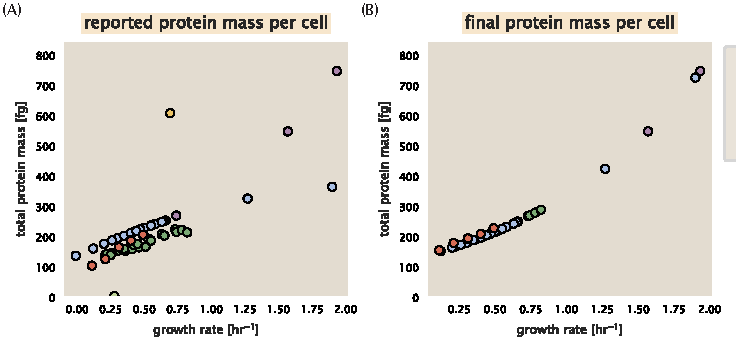
\includegraphics[width=1\textwidth]{../../figures/dataset_corrections.pdf}
  \caption{}
  \label{fig:dataset_correlations}
\end{figure}


\section{Adjustments to Copy Number Data.}

% NB: need to make summary figure with 2x2 panels; top row A) reported total protein per cells
% B) protein concentration. bottom row, C) new total protein mass per cell,
% C) new protein concentration.

% NB: It may be helpful to appeal to the 'classic growth laws' early on in this text
% as a rational to guide thinking with expectations about total cell mass, cell volume w.r.t.
% growth rate.

The datasets encompass a range of bacterial growth conditions,  different {\it
e. coli} strains, and for those that report quantities on a cell basis,
different methods to normalize  by  cell count and volume. It was therefore
important to consider if certain discrepancies exist across the data and whether
these might be reasonably dealt with to make the compilated dataset internally
consistent. - give reference to what was done in example of yeast proteome data
corrections. However, given the work of [cite] and others, there are
well-documented expectations about how characteristics such as total protein
mass per cell and cell volume  should scale with growth rate. We were therefore
inclined to only renormalize data in a  way  that took into account such
expectations. Figure \ref{} shows the total protein  mass reported as a function
of growth rate for each experiment. Indeed, with the exception of the work of
Peebo et al., the total mass per cell is generally consistent as a function of
growth rate, and provide some confidence in such an approach.

In the remainder of this section we describe the rescaling that was done to each
dataset, with a particular focus on correcting for discrepencies in cellular
protein concentration, which may reflect differences in protein extraction
efficiency. It is important to note that with the exception of the work from
Peebo {\it et al.} (which is discussed more below), any rescaling is only
performed within the data of individual authors and not performed globally. We
felt this was important in order not to bias any individuals' work since we lack
any true standard of protein abundance.

% for differences in
% cellular protein concentration within each inidividual dataset. This  strategy
% was already applied in the work of Schmidt et al., in particularr due to
% concerns  over lower protein extraction efficiency in growth conditions like
% stationary phase.  However, another complicating factor that became apparent is
% a descrpency in expected versus reported cell volume that required additional
% care and is further described below. Lastly, the  data from Peebo {\it et al.}
% required additional care due to a lack quantities on a cell basis, and we
% consider this work separately.


\subsection{Corrections to Enforce a Consistent Cellular Protein Concentration}

% NB: It may be useful to note that none of this should have any effect on the relative
% abundances found in each dataset.

One parameter that we do not expect to change substantially across growth
conditions is cellular protein concentration. As a general rule of thumb, we
expect an {\it e. coli} cell to have about 30\% dry mass, with about 55\% of
this expected from protein. With a density of about 1.1 g/ml, we find that the
protein concentration in a cell should be approximately 180 fg/fL.  The cellular
density and dry mass are essentially fixed, with the fraction of cellular
protein varying from [X-Y; refs??]. Hence,  this parameter provides a useful
reference point that datasets should agree on.  Indeed, out of concern over
differences in protein extraction efficiency in growth phases like stationary
phase, Schmidt {\it et al.} applied a correction to their measured protein
abundances to ensure cellular protein concentrations were internally consistent.


From the work of Schmidt {\it et al.} they reported an ability to consistently get high
protein yield from cells grown in M9 minimal media supplemented with glucose. In order
to account any protein loss during extraction, they use their measured protein concentration
from this sample as a reference for which total protein concentration in all other growth
conditions should match. This is shown in Figure \ref{}A. One challenge in
performing this calculation is that cell volume must be known; the authors use
volumes that were  measured by flow cytometry in previous work [cite]. These
volumes are shown in Figure \ref{}B. While it is difficult to assess the
accuracy of these numbers, we find them to be quite inconsistent with the
expected scaling that is reported by Taheri-Araghi {\it et al.} (2015),
carefully
measured as a function of growth rate [and other work?].

In addition, since cell volume was not determined in all studies, and to be
consistent throughout, we instead use the predicted cell volumes from
Taheri-Araghi {\it et al.}. Dealing with each dataset seperately, we apply
correction  factors to correct for discrepencies in protein concentration across
the different growth conditions considered [NB: I wonder if in these other
datasets, the more appropriate thing to do is match to the average measured
protein concentration]. Specifically, the scaling factor $\phi$ is given by,

\begin{equation}
\phi  =  \frac{P_i}{V_i} \cdot [P]_r
\end{equation}

where $P_i$ is the total protein mass in conditino $i$, $V_i$ is the estimated cell volume, and $[P]_r$ is
the reference protein concentration (i.e. growth in  glucose for the Schmidt data).


\subsection{Peebo {\it et al.}: Conversion from copies/ fL to copies per cell}

In the work of Peebo {\it et al.}, the authors only report protein concentration.
In  order to determine protein per cell, we multiple these concentrations by
expected cell volumes  using the predictions from  Taheri-Araghi {\it et al.} This is
shown in Figure \ref{}A, where we see that reported mass is substantially lower than
the other work considered here; as well as work from others [Sinauer, 1990].

Indeed, both Schmidt {\it et al.} and Li {\it et al.} reported a total protein mass of about
250 fg per cell at a growth rate of about $\lambda \approx 0.5 hr^{-1}$ ( M9
minimal media with glucose and MOPS minimal media, respectively). Given this
discrepancy, in addition to requiring that cellular protein concentration be
internally consistent across the growth conditions they reported on, we also
required that total cellular mass be consistent with the work Schmidt {\it et al.} and
Li {\it et al.} This amounted to performing a linear regression between total protein
mass and growth rate, and using this to scale the Peebo {\it et al.} dataset according
to this trend.


 % cell biology by the numebrs: Overall macromolecular composition of an average
 % E. coli cell in aerobic balanced growth at 37°C in glucose minimal medium,
 % with doubling time of 40 minutes and 1 pg cell wet weight (≈0.9 μm^3 cell
 % volume). Adapted with modifications from F. C. Neidhardt et al., “Physiology
 % of the bacterial cell”, Sinauer, 1990 (BNID 104954). Modifications included
 % increasing cell dry weight from 284 fg to 300 fg and total cell mass from 950
 % to 1000 fg as

%
\newpage
\section{Translation-dependent limits on the rate of cell division.}

Here we consider the hypothesis that the process of translation sets the speed
limit of bacterial growth. We begin by considering the synthesis of the ribosome
itself, finding that it sets a strict limit on division time, and then from there we
consider how the remaining proteome further limits this achievable growth rate.

\subsection{Maximum possible growth rate is set by the time to make a ribosome.}

\marginnote{\small{NB: This time is longer if we need to add in e.g. elongation
factors as a 'core' protein to replicate a ribosome. RP to NB: rRNA estimate can
also go here.}}

Ribosomes take a unique position among proteins due to their role in
synthesizing the entire cellular proteome. In order for a cell to maintain its
own pool of ribosomes during division into two daughter cells, a primary
requirement is that the number of ribosomes must be doubled.  Since the  mass of
a single ribosome is about 2.5 MDa, with about 2/3 RNA and 1/3 protein, each
ribosome has to make about 800 kDa of protein. In {\it E. coli},
this corresponds to 7,459 amino acids. At a maximal translation rate of 20 amino
acids per second, this would take just over 6 minutes.  Growing any faster would
result in a drop in the average number of ribosomes as the cell divides and
highlights a strict time limit on how fast a cell can double itself.  This
result is irrespective of the absolute number of ribosomes, and contrasts with
other proteins where the simple solution to making more proteins is to
apparently devote more ribosomes to their synthesis.

\subsection{The translation-limited growth rate is set by the fraction of
ribosomal mass.}

While the inability to parallelize ribosomal synthesis sets an inherent speed
limit, this also represents a somewhat unachievable growth rate since ribosomes must
spend some of their time doubling the remaining proteome. A
translation-limited rate of growth is therefore set by the time to double the
entire proteome. In order to understand the consequence of each ribosome having
to duplicate itself, but also devote time to double the remaining proteome, we
consider a hypothetical cell that consists of only two species of protein:
ribosomes and non-ribosomal proteins. The cell is taken to contain $R$ ribosomes
per cell, and $P$ non-ribosomal proteins per cell. The time $\tau$ needed to
duplicate the entire proteome is simply given by,


% The only way to reach the minimum duplication time
% set by the ribosome would be to increase the relative fraction of ribosomes.
% This would effectively reduce the time needed to duplicate the non-ribosomal
% proteins.

\begin{equation}
	\tau = \tau_R + \tau_P,
\label{eq:tau}
\end{equation}
where $\tau_R$ is the time to double the ribosome copy number and $\tau_P$ is the time
required to double the non-ribosomal proteins. While we found that $\tau_R$ is fixed
at about 6 minutes,  $\tau_P$  will depend on the number of ribosomes $R$ available and
can be approximated by,

\begin{equation}
\tau_P = \frac{N_{aa}}{r_t \cdot R}.
\label{eq:tau_P}
\end{equation}
Here $N_{aa}$ refers to the total number of amino acids (aa) that must be
translated, while $r_t$ refers to the elongation rate of translation.
The translation-limited growth rate can then be calculated from,

\begin{equation}
\lambda_{\text{max}} =  \frac{ln(2)} {\tau}.
\end{equation}
Using Equation \ref{eq:tau_P} and \ref{eq:tau}, this becomes,
\begin{equation}
\lambda_{\text{max}} =  \frac{ln(2)} {\tau_R + \frac{N_{aa}}{r_t \cdot R}}.
\label{eq:lambda_max}
\end{equation}
We can see from Equation \ref{eq:lambda_max} that the only way to increase the
translation-limited growth rate would be to make more ribosomes, or if it were
possible, to decrease the number of non-ribosomal proteins. For now we will assume
that the translation elongation rate is fixed at about 20 aa/s but will return to this
assumption in a later section.

let's now use some representative values for $R$ and $N_{aa}$ to calculate
$\lambda_{\text{max}}$. From Schmidt {\it et al.}, cells grown in glucose were
found to have 214 fg of non-ribosomal  protein mass \cite{Schmidt2016}. Taking
the molecular weight of an average amino acid to be 110 g/mol and using Avogadro's number $N_A$, we can estimate
$N_{aa}$ = 214 x 10$^{-15}$g / (110 g/mol) x $N_A$,
which corresponds to about 1x10$^9$ amino acids.  Similarly, we can use their
reported ribosomal mass of about 29 fg to estimate the ribosomal copy number,
$R$. With a molecular weight of about 800 kg/mol as noted earlier,  $R$ =
29 x 10$^{-18}$kg / (800 kg/mol) x $N_A$,   which we find to be about 22,000 per
cell. Using Equation \ref{eq:lambda_max}, this corresponds to a maximum growth
rate of 0.8 hr$^{-1}$, versus the measured rate of 0.58 hr$^{-1}$, suggesting
cells are growing slightly below their maximal rate.

Since the only way to divide faster than this limit set at 0.8 hr$^{-1}$ would be
for the cell to increase the number of ribosomes, we next consider how
growth rate might vary as a function of ribosomal copy number. To
keep our problem simple,  lets first proceed with the simplifying assumption
that our cell consists of  214 fg of non-ribosomal protein, and consider
how $\lambda_{\text{max}}$ varies  as a function of the ribosome copy number $R$
using Equation \ref{eq:lambda_max}.  While in reality we might expect other
proteins to increase in proportion to the number of ribosomes, this calculation
provides us with a bound on the maximum growth rate as a function of $R$.  In
Figure \ref{fig:estimates_translation_toy_1} we consider the range of experimentally observed values
of $R$ from about 10,000 copies per cell to
150,000 copies per cell. One observation is that
the maximum growth rate is always less than that set by the synthesis time of a
ribosome, at about 3 hr$^{-1}$ when $R$ is 150,000 ribosomes per cell. Indeed, while not shown,
we find that $R$ would need to be increased another 10 fold, to
about one million copies per cell, to have a doubling time close to that set by the ribosome (with a 6 minute ribosome synthesis time
corresponding to a growth rate of about 7 hr $^{-1}$).

% One difficultly that
% arises is that in order for a cell to add more ribosomes, it will need to
% increase in size. This might require that other proteins also increase in number to
% maintain a specific proportion relative to the cell size. However,
% that the value of $N_{aa}$ is sufficient to
% build a cell irrespective of the number of ribosomes.
% This in effect provides us with a
% lower bound on the total proteomic content at faster growth rates and a lower
% limit on the achievable growth rate.

\begin{figure}[H]
		\centering
    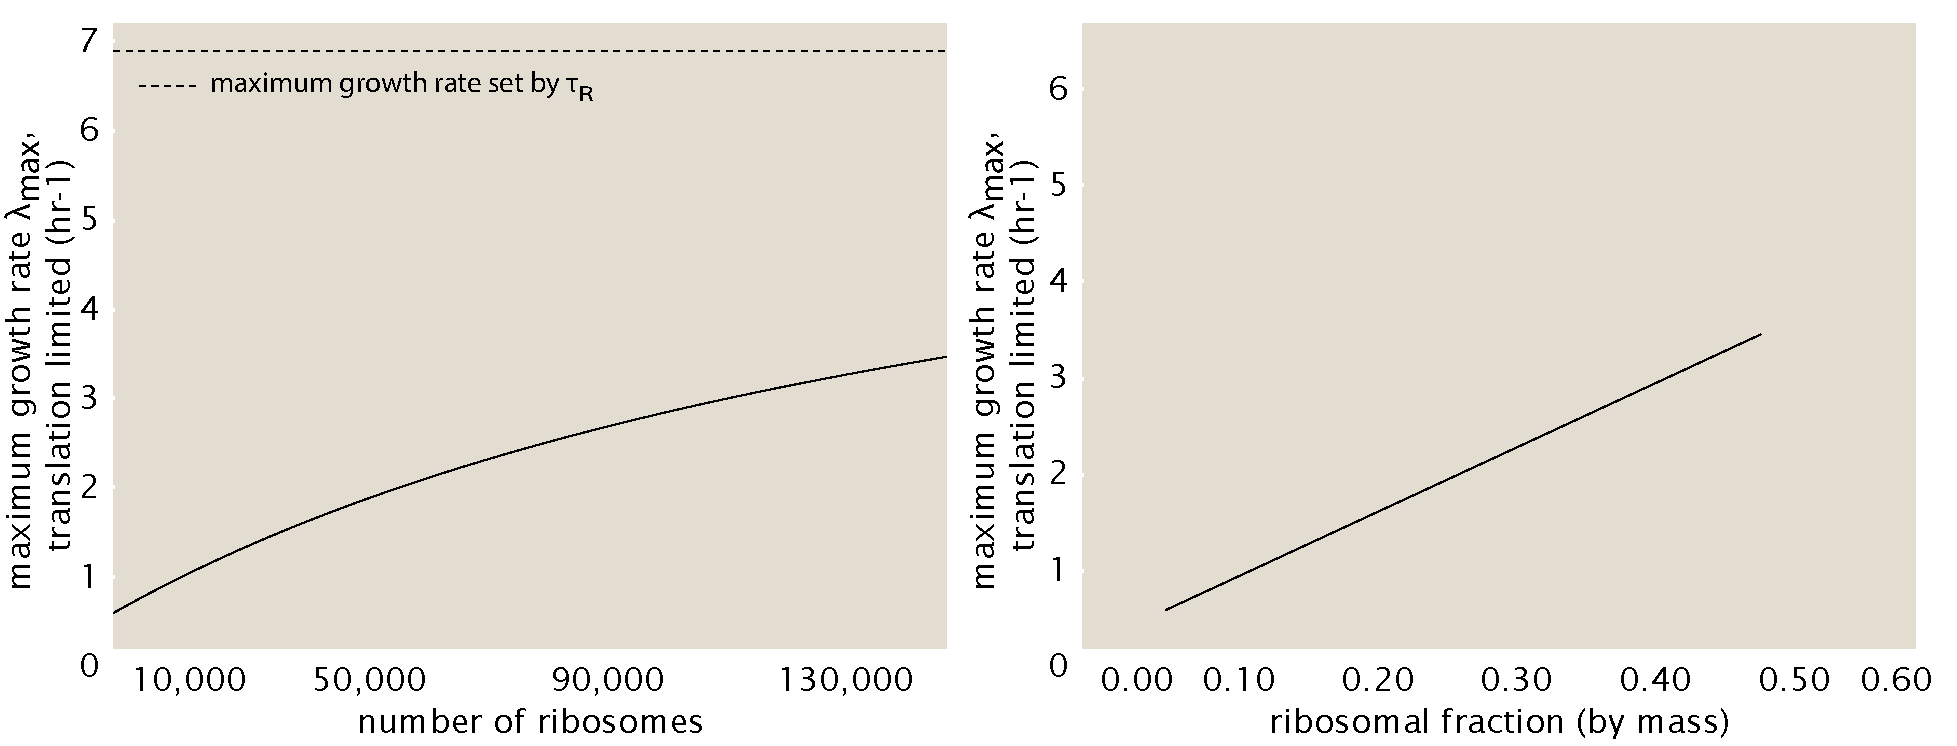
\includegraphics[width=1\textwidth]{../../code/figures/SI/estimates_translation_toy_1.pdf}
  \caption{{\bf Expectations on the maximum growth rate as a function of ribosome abundance.}
	 	A) Plot of the translation-limited growth rate in Equation
	 	\ref{eq:lambda_max}, with $N_{aa}$ = 1.2 x 10$^9$ amino acids, and $R$ from about
	 	10,000 to 150,000 copies per cell. B) Related to part A, but instead
	 	showing the translation-limited growth rate as a function of ribosomal mass
	 	fraction.}
  \label{fig:estimates_translation_toy_1}
\end{figure}

Given how many ribosomes a cell would need in order to double a cell in 6 minutes,
it is also useful to consider what this might mean with
respect to cell size. Note that cell volume will be proportional to cell mass.
We can estimate a lower bound on the required cell volume as a function of the
$R$ by assuming a mass density of 1.1 g/ml, and a dry mass of 30\% consisting of
only protein and RNA. This is plotted in Figure
\ref{fig:estimates_translation_volume}, where we've extended the range of $R$ up
to about one million copies per cell. While we find cell volumes consistent with our expectation for {\it E. coli}
for values of $R$ less than about 100,000 per cell, the plot also highlights that a cell would need to be
excessively largem with a minimal volume of about 25 $f$L, in order for
$\lambda_{\text{max}}$ to be close to the 6 minute doubling time set by the ribosome.

\begin{figure}[H]
		\centering
    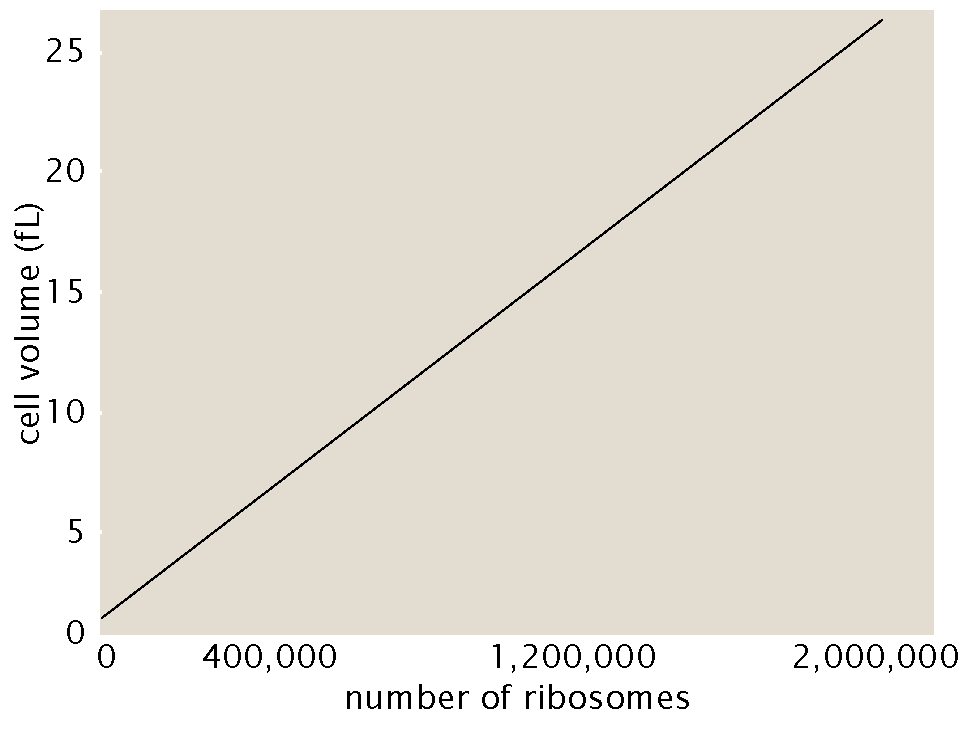
\includegraphics[width=0.5\textwidth]{../../code/figures/SI/estimates_translation_volume.pdf}
  \caption{{\bf Estimated scaling of cell size with ribosomal copy number.} As a first approximation,
	the cell mass it taken to consist of 214 fg non-ribosomal protein, and a ribosomal mass based
	on 1/3 corresponding to protein, and 2/3 corresponding to RNA. The cell volume is then calculated assuming
	a 30 \% dry mass, and cell mass density of 1.1 g/ml. }
  \label{fig:estimates_translation_volume}
\end{figure}

As a last consideration, one additional observation from Figure \ref{fig:estimates_translation_toy_1}B
is an apparently linear dependence
between $\lambda_{\text{max}}$  and the fraction of ribosomal mass. This, along with the
scaling in ribosomal copy number, are particularly relevant to the
phenomenological growth laws reported by others on how cell size and cell mass
scale with growth rate in bacteria. The linear scaling appears to be a feature
irrespective of the size of the non-ribosomal mass, as shown in Figure
\ref{fig:estimates_translation_ribo_frac}. Indeed, with a bit of algebra, we can
re-write the translation-limited growth rate defined by Equation
\ref{eq:lambda_max} as a function of ribosomal mass fraction, denoted by
$\Phi_R$, as,

\begin{equation}
\lambda_{\text{max}} =  \frac{ln(2)} {L_R} \cdot r_t \cdot \Phi_R.
\label{eq:lambda_max_phi}
\end{equation}
$L_R$ refers to the number of amino acids that make a single
ribosome ($L_R$ = 7,459 aa for a complete ribosome in {\it E. coli}). As a sanity check, we can quickly
see that if $\Phi_R$ = 1, we are once again limited only by the time required to
double a ribosome $L_R / r_t$.

\begin{figure}[H]
		\centering
    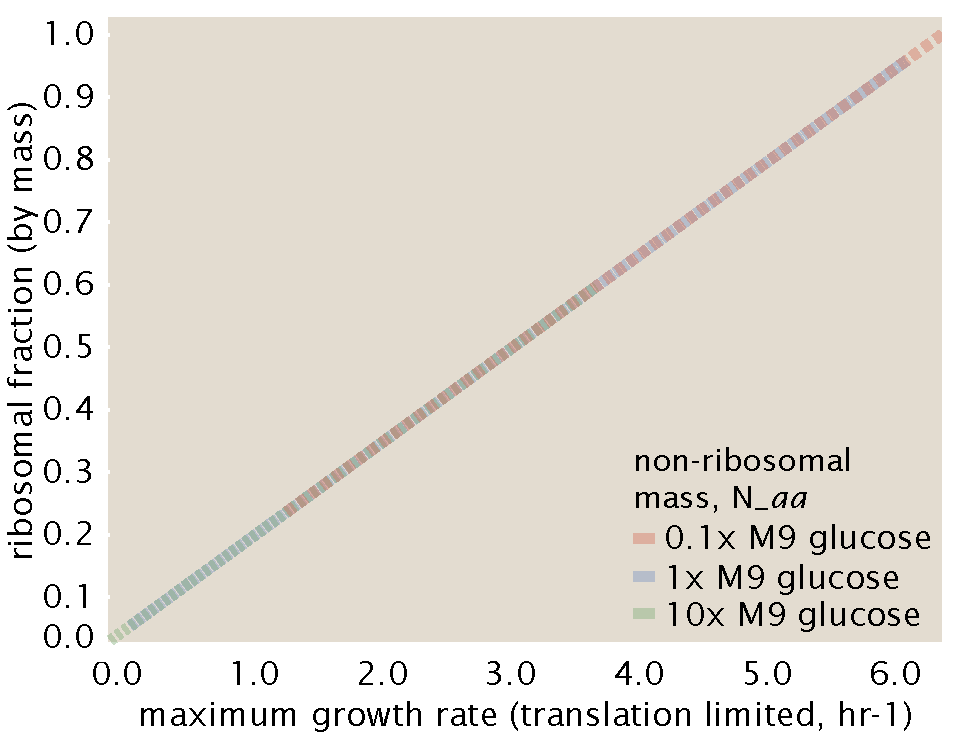
\includegraphics[width=0.5\textwidth]{../../code/figures/SI/estimates_translation_ribo_frac.pdf}
  \caption{{\bf Effect of ribosomal mass fraction on translation-limited growth rate.} Following the approach
	result from Figure \ref{fig:estimates_translation_toy_1}B, we recalculate the maximum growth rate as
	the total non-ribosomal mass is either reduced or increased ten-fold (i.e. $N_{aa}$ = [0.1x$N_{aa}$, $N_{aa}$, 10x$N_{aa}$]).}
  \label{fig:estimates_translation_ribo_frac}
\end{figure}


\subsection{Growth only appears translation-limited in rich growth media.}

With an expectation on the maximum growth rate achievable as a function of
ribosomal content from our discussion above, lets now take a look at our experimental
data. From Equation \ref{eq:lambda_max_phi}, we found that the
translation-limited growth  rate is simply determined by the fractional
ribosomal mass $\Phi_R$ which we can easily calculate from our proteomic data.   In Figure
\ref{fig:estimates_translation_data}A we plot this maximal growth rate,
$\lambda_{\text{max}}$, against the measured growth rates, while in Figure
\ref{fig:estimates_translation_data}B we plot the cell cycle or doubling time that would be
associated with these growth rates. The shaded regions identify regions that
should not be attainable with a translation elongation rate $r_t$ of 20 aa/s.
From these two plots, it appears that cells are only translation-limited in rich
media (data points with growth rates greater than $\approx$ 1 hr$^{-1}$ in Figure
\ref{fig:estimates_translation_data}A)).

% \marginnote{\small{NB: A better way would be to directly calculate the number of
% aa from proteomic sequences and copy number.}}

% \marginnote{\small{NB: There is something weird about the fraction of ribosomal
% protein in Peebo, Valgepea; it is higher, and also higher than that found in Scott
% {\it et al.}  - is it real??}}

\begin{figure}[H]
		\centering
    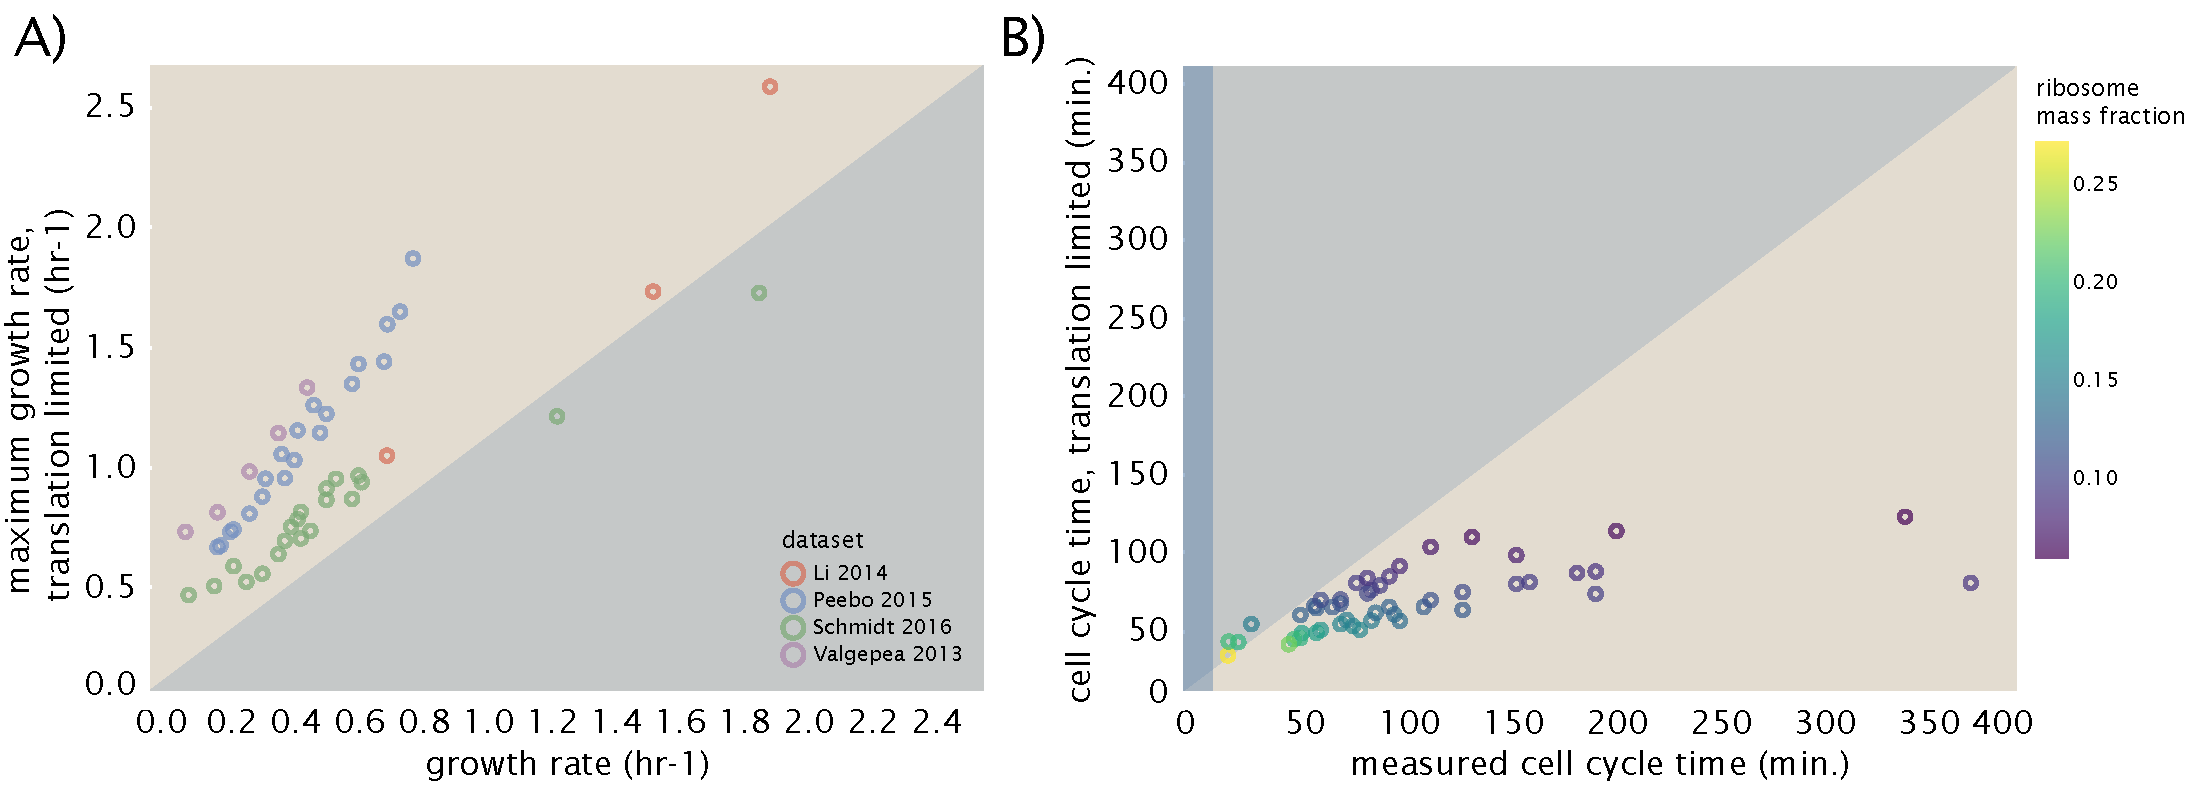
\includegraphics[width=1\textwidth]{../../code/figures/SI/estimates_translation_data.pdf}
  \caption{{\bf Comparison of translation-limited rate of growth to observed growth rates.}
	A) Plot of maximum growth rates based on reported cell mass and calculated from Equation \ref{eq:lambda_max}.
	B) Related to (A), but instead plotting the cell cycle time in minutes.
	The light shaded regions in (A) and (B) reflect boundaries where growth would not be possible
	due to a translation rate of 20 aa/s. The dark shaded region in (B) corresponds to the maximum
	division rate set by doubling a ribosome.
	(\smaller{NB: There is something weird about the fraction of ribosomal
	protein in Peebo, Valgepea; it is higher, and also higher than that found in Scott
	{\it et al.}  - is it real??})}
  \label{fig:estimates_translation_data}
\end{figure}

\subsection{The effect of a non-constant translation elongation rate.}

From Figure \ref{fig:estimates_translation_data}B it is apparent that for cells
with slower growth, the cell cycle time is indeed much longer than might have
been expected under translation-limited growth. The remaining parameter we have yet to
consider is the elongation rate $r_t$, which we have assumed to be 20 aa/s. Recent
measurements of elongation rate from Dai {\it et al.} \cite{Dai2016} across a
wide range of growth rates found that it indeed varies with growth rate. In particular,
they showed that the rate decreased to as low as 8 aa/s and exhibited a a Michaelis–Menten dependence on the
ribosomal fraction. Here we use their result to further consider the consequence of a
decreasing elongation rate $r_t$ on the maximum predicted growth rate.

% We can actually infer what
% the effective translation is given the observed growth rates, which we show
% in Figure \ref{fig:estimates_translation_rate}.  Interestingly, these
% translation rates are in good agreement with those measured in Dai {\it et al.}
% \cite{Dai2016}, which were also shown to decrease when grown under limited nutrient conditions.
%
% \marginnote{\small{JT suggests using measured elongation rate in Dai {\it et al.} to redefine
% translation boundaries in Figure \ref{fig:estimates_translation_data}.}}
%
% \begin{figure}[H]
% 		\centering
%     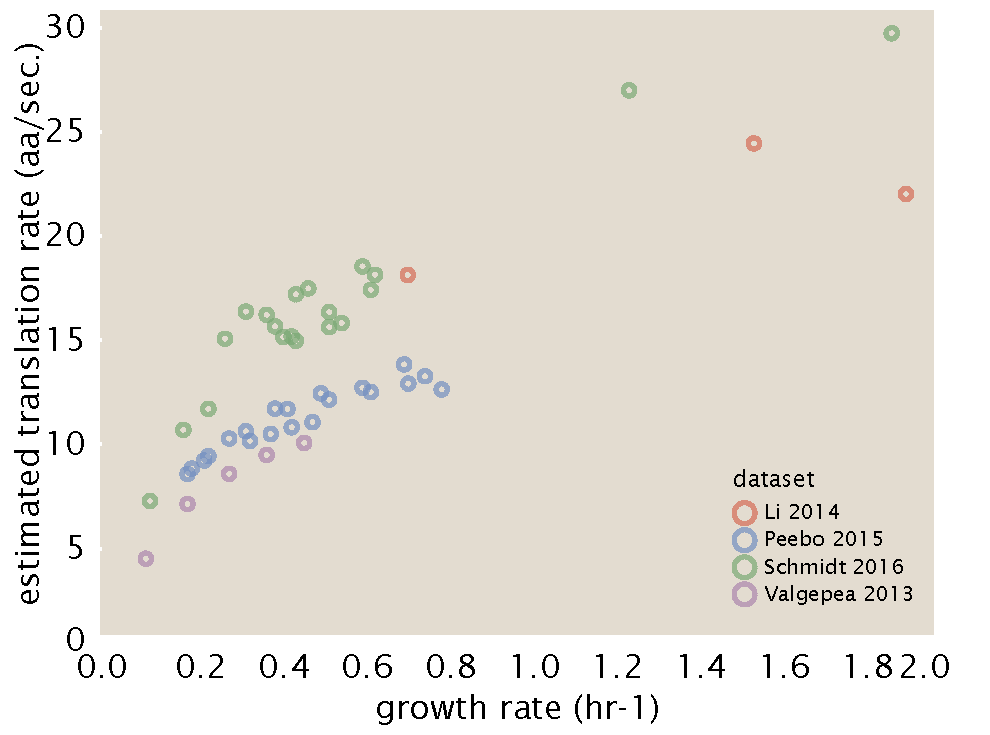
\includegraphics[width=0.5\textwidth]{../../code/figures/SI/estimates_translation_translation_rate.pdf}
%   \caption{{\bf Estimate of apparent translation rates based on observed growth rates and measured proteomic mass.}
% 	Using the measured ribosomal and non-ribosomal mass, we use Equation \ref{eq:lambda_max}  to estimate $r_t$
% 	for each of the proteomic datasets available.}
%   \label{fig:estimates_translation_rate}
% \end{figure}

\marginnote{\small{NB: a better approach would be from
point-of-view of biological rate-limiting steps. BUT the result suggests possibilities: aa-tRNA availability?,
GTP?}}

In the work of Dai et al. the authors propose that there may be a bottleneck in
translation that arises due to lower  availability of ternary complex (TC)
that must bind the ribosome in order for translation to proceed. This complex
consists of aminoacyl-tRNA, elongation factor Tu and guanosine triphosphate.
To account for this bottleneck, they divide the elongation rate into two
coarse-grained timescales: A) binding of the ternary complex to the ribosome,
which will depend inversely on the effective TC concentration $[TC_{eff}]$, and
B) other enzymatic processes that will not depend
on TC concentration. Letting these two timescales be 1/($k_{on} \cdot
[TC_{eff}]$) and 1/$r_t$, the new elongation rate is given by,

\begin{equation}
\frac{1}{r_t'} = \frac{1}{k_{on} \cdot [TC_{eff}]} + \frac{1}{r_t}
\label{eq:rate_dai}
\end{equation}
where $r_t/k_{on}$ is the binding constant of the TC with the ribosome. Further
taking $[TC_{eff}]$ to be proportional to the RNA/protein ratio,

\begin{equation}
[TC_{eff}] = C \cdot (R_m/P_m),
\label{eq:elong_rate}
\end{equation}
they find that  $r_t$ = 22 aa/s, $k_{on}$ = 6.4 $\mu M^{-1}s^{-1}$, and
$C$ = 31 $\mu M$.

\marginnote{\small{This assumption of proportionality
is something that will need some more consideration.}}

Using the elongation rate calculated from Equation \ref{eq:elong_rate}, we can now
recalculate the translation-limited growth rate,

\begin{equation}
\lambda_{\text{max}}' =  \frac{ln(2)} {L_R} \cdot r_t' \cdot \Phi_R,
\label{eq:lambda_max_phi_dai}
\end{equation}
where we denote $\lambda_{\text{max}}'$ as the translation-limited growth rate when elongation rates is no longer assumed
to be fixed at 20 aa/s. Plugging in the translation rate $r_t'$ given by Equation \ref{eq:rate_dai}
along with the measured fraction of ribosomal mass $\Phi_R$ from each dataset, we find a
further improvement in agreement between the measured and translation-limited growth rates.
This is shown in Figure \ref{fig:estimates_translation_data_dai}. This is particularly true with
the data from Li {\it et al.} and Schmidt {\it et al.}, though we note that
for the poorest nutrient conditions (i.e. the longest cell cycle time) a
discrepancy still appears to exist.

\begin{figure}[H]
		\centering
    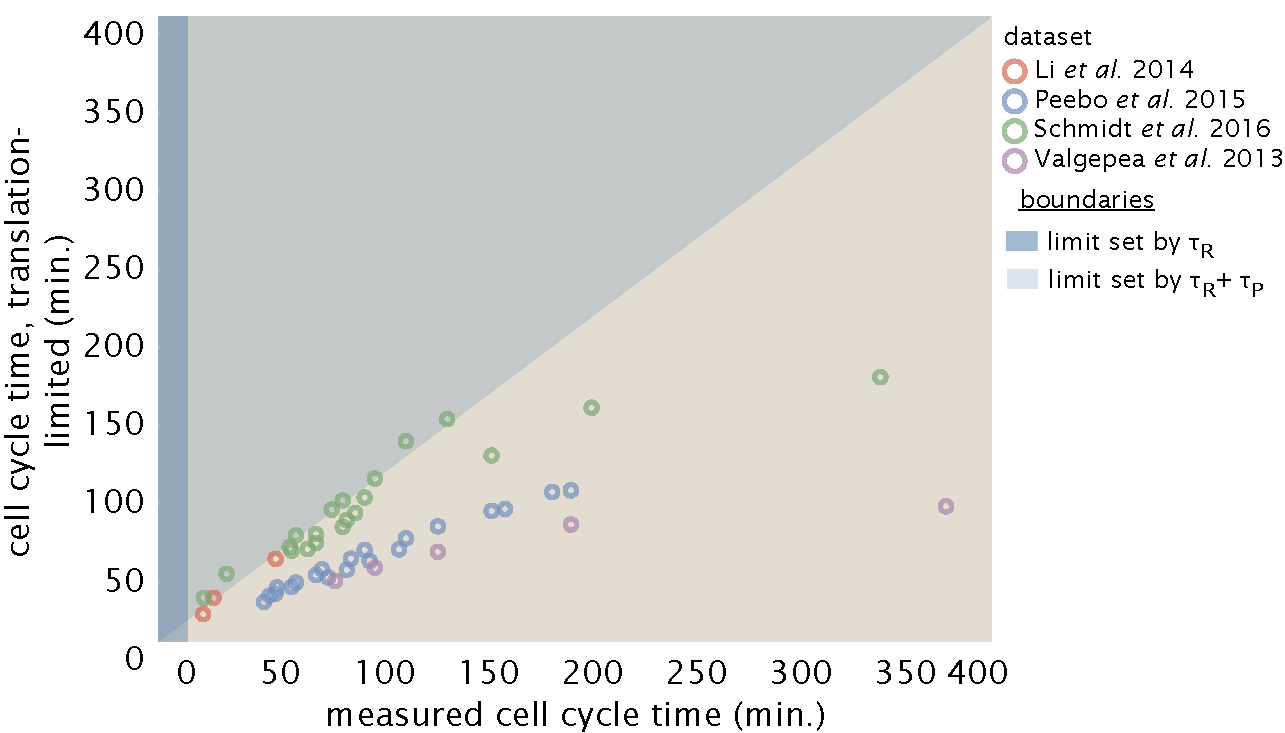
\includegraphics[width=0.7\textwidth]{../../code/figures/SI/estimates_translation_data_dai.pdf}
  \caption{{\bf Comparison of translation-limited rate of growth to observed growth rates using the predicted
	elongation rate from Dai {\it et al.}.}
	Predicted cell cycle time, calculated from  Equation \ref{eq:lambda_max_phi}, is plotted
	against the measured doubling time.	The light shaded region reflect a boundary where growth would not be possible
	given the predicted translation rate $r_t'$ in Equation \ref{eq:rate_dai}, which varies from about 8 aa/s to about 20 aa/s.
	The dark shaded region corresponds to the maximum
	division rate set by the synthesis of a ribosome. To calculate the RNA/ protein ratio
	$R_m/P_m$ we assume it is proportional to the fraction of ribosomal mass $\Phi_R$,  which
	empirically was found to be $R_m/P_m$ = $\Phi_R$/0.411 \cite{Dai2016}.}
  \label{fig:estimates_translation_data_dai}
\end{figure}

\bibliography{SI_bib.bib}

\end{document}
